\documentclass[12pt]{article}
\usepackage[a4paper, total={6in, 8in}]{geometry}
\usepackage{amsfonts}
\usepackage{amsmath,amssymb,trimclip,adjustbox}
\usepackage{polski}
\usepackage{tabularray}
\usepackage{tabularx}
\usepackage[utf8]{inputenc}
\usepackage[x11names]{xcolor}
\usepackage{tcolorbox}

\newtcolorbox{tw}[1]{colback=Green4!5!white,
colframe=Green4!75!black,fonttitle=\bfseries,
title={#1}}

\newtcolorbox{blad}[1]{colback=red!5!white,
colframe=red!75!black,fonttitle=\bfseries,
title={#1}}

\newtcolorbox{przyklad}{colback=white, fonttitle=\bfseries, title={Przykład}}
\newtcolorbox{przykladbig}{colback=white, fonttitle=\bfseries, breakable, title={Przykład}}

\newcommand{\bbk}{\mathbb{K}}

\setlength{\parindent}{0pt} 
\setlength{\textheight}{680pt}
\setlength{\oddsidemargin}{-15pt}
\setlength{\textwidth}{480pt}

\everymath{\displaystyle}

\author{Michał Puchyr}
\date{}
\title{Notatki na kolokwium z Matematyki dyskretnej -- część 2}

\begin{document}

\maketitle

\section{Relacje równoważności}

\begin{tw}{Objaśnienia}
    Operacja rozbicia - rozdzielanie klas równoważności np. $ \{a,b,c\} \overset{op2}{\to} \{a,b\} \{c\} $
    
    Operacja sklejenia - sklejanie klas równoważności np. $ \{ a, b \} \{c\} \overset{op1}{\to} \{a,b,c\} $
    \medskip
    
    Operacja odłączania - op3 przekształca podział w taki sposób, że usuwa część lub wszystkie obiekty z wybranej klasy podziału i lokuje
    je w specjalnym buforze pomocniczym. Jeśli bufor pomocniczy jest niepusty, obiekty są do niego dodawane.
    \medskip

    Operacja dołączania - op4 przekształca podział w taki sposób, że usuwa część lub wszystkie obiekty z bufora pomocniczego i dołącza
    je do istniejącej klasy podziału albo tworzy z nich nową klasę podziału.
\end{tw}

\begin{przyklad}
    Niech dany będzie zbiór $U = {u_1, u_2, ... , u_{10}}$ oraz relacje równoważności $P, Q \in \mathbb{E}(U)$
    reprezentowane podziałami:
    \[\mathbb{K}_P = \{\{u_1, u_2, u_3\}, \{u_4\}, \{u_5, u_6\}, \{u_7, u_8, u_9, u_{10}\}\}\]
    \[\mathbb{K}_Q = \{\{u_1\}, \{u_2, u_3, u_4, u_5\}, \{u_6\}, \{u_7, u_8\}, \{u_9, u_{10}\}\} \]
    Oblicz $\delta^{1,2}$ (P, Q) oraz $\delta^{3,4}$ (P, Q).

    Rozwiązanie
        \begin{enumerate}
            \item $\delta^{1,2} = 4 lub 6$
            \item $\delta^{3,4} = 4$
        \end{enumerate}
    
\end{przyklad}

\section{Aproksymacje}

\begin{tw}{Przybliżenie zbioru}
    Mówimy, że dla zadanego uniwersum $U$, określona została przestrzeń aproksymacyjna $ \bbk = {K_1, K_2, ..., K_M} $, wtedy i tylko wtedy
    gdy $ \bigcup_{i = 1}^{M} \ K_i = U $ \ oraz \ $ K_i \cap K_j = \varnothing $ \ dla \ $ i \neq j $. Przybliżeniem zbioru $ D \subseteq U $
    w przestrzeni aproksymacyjnej $\bbk$ (określonym także terminem zbiór przybliżony) nazywamy parę:
    \[ \text{apr}(D) = (\text{apr}_{\bbk}, \text{apr}^{\bbk}(D)) \]
    gdzie
    \[ \text{apr}^{\bbk} (D) = \bigcup_{K \in \bbk, \ K \cap D \neq \varnothing } K \hspace{50pt} \text{apr}_{\bbk}(D) = \bigcup_{K \in \bbk, \ K \subseteq D} K \]

    $ \text{apr}^{\bbk}(D) $ -- przybliżenie zbioru $ D $ z góry

    $ \text{apr}_{\bbk}(D) $ -- przybliżenie zbioru $ D $ z dołu
\end{tw}

\begin{tw}{Miary jakości przybliżenia}
    \[ \text{completness}(\text{apr}(Z)) = \frac{ |\text{apr}_{\bbk}(Z)| }{|Z|} \]
    \[ \text{precision}(\text{apr}(Z)) = \frac{ |\text{apr}^{\bbk}(Z)| }{|Z|} \]
\end{tw}

\begin{przyklad}
    Niech $ U = \{u_1, u_2, u_3, u_4, u_5, u_6, u_7\} $ \ oraz niech $\bbk = \{ \{ u_1, u_2 \}, \{ u_3, u_4, u_5 \}, \{ u_6, u_7 \} \}$
    Wyznaczyć dolną i górną aproksymację dla $ Z_2 = \{ u_1, u_2, u_3, u_4 \} $.

    \begin{center}
        \begin{tabular}{c|c|c}
            $ K_i $ & $ K_i \cap Z_2 $ & $ K_i \subseteq Z_2 $ \\
            \hline
            $ \{ u_1, u_2 \} $ & $ \{ u_1, u_2 \} $ & $ \{ u_1, u_2 \} $ \\
            $ \{ u_3, u_4, u_5 \} $ & $ \{ u_3, u_4 \} $ & $ \varnothing $ \\
            $ \{ u_6, u_7 \} $ & $ \varnothing $ & $ \varnothing $ \\
        \end{tabular}
    \end{center}

    \[ \text{apr}_{\bbk}(Z_2) = \{ u_1, u_2 \} \]
    \[ \text{apr}^{\bbk}(Z_2) = \{ u_1, u_2, u_3, u_4 \} \]

    Obliczyć kompletność i miarę jakości przybliżenia dla $Z_2$.
    \[ \text{completness}(\text{apr}(Z_2)) = \frac{ |\text{apr}_{\bbk}(Z_2)| }{|Z_2|} = \frac{2}{4} = 0.5 \]
    \[ \text{precision}(\text{apr}(Z_2)) = \frac{ |\text{apr}^{\bbk}(Z_2)| }{|Z_2|} = \frac{4}{4} = 1 \]
\end{przyklad}

\begin{blad}{Aproksymacje - Na chłopski rozum}
    Przybliżenie dolne - jest to zbiór elementów, które w całości zawierają się w zbiorze przybliżanym.

    Przybliżenie górne - zbiór wszystkich elementów, które mają chociaż jeden element wspólny z przybliżanym zbiorem.

    Przybliżenie odgórnie równe jest wtedy kiedy przybliżenia górne zbiorów są takie same. Zapis $ X = ^{\bbk}Y $

    Przybliżenie oddolnie równe jest wtedy kiedy przybliżenia dolne zbiorów są takie same. Zapis $ X = _{\bbk}Y $

    Zbiory równe w przestrzeni aproksymacyjnej $ \bbk $ wtedy i tylko wtedy gdy $ X = ^{\bbk}Y $ oraz $ X = _{\bbk}Y $. Piszemy $ X = \frac{\bbk}{\bbk}Y $
\end{blad}

\section{Wyznaczanie reprezentanta}

Różnica symetryczna zbiorów $A$ i $B$ to zbiór elementów należących do $A$ lub $B$, ale nie należących do $A \cap B$.

\begin{center}
    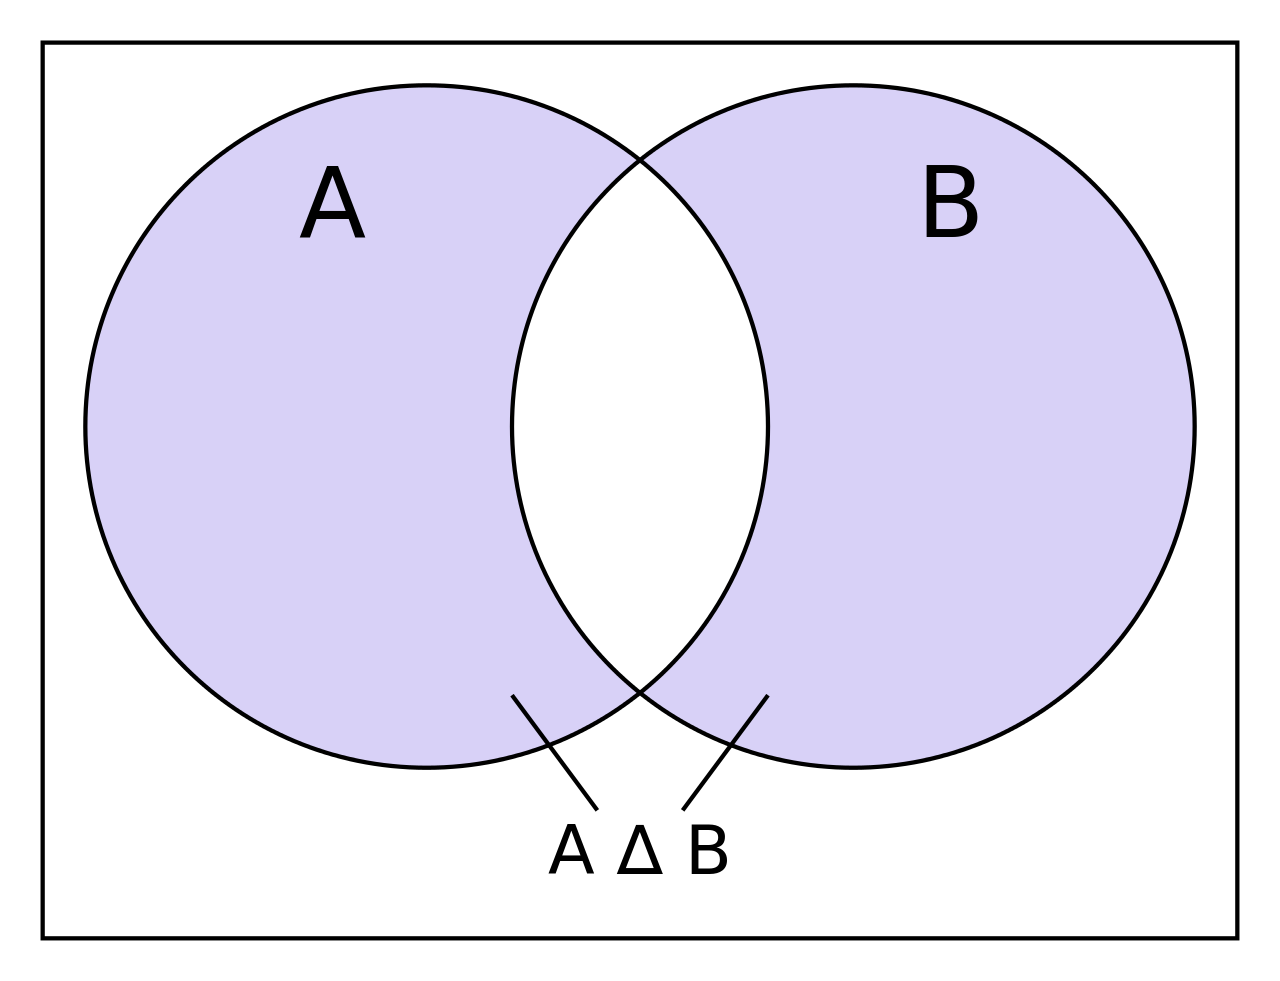
\includegraphics[scale=0.1]{roznicasymetryczna.png}
\end{center}

Do wyznaczania podobieństwa można użyć wzór 
\[ \sigma = \frac{1}{1 + \delta} \]

\begin{przyklad}
    Niech dane będzie uniwersum $U = \{a, b, c, d, e, f\}$ z funkcją odległości
    $\delta : U \times U \to R+$ jako makrostrukturą:

    \begin{center}
        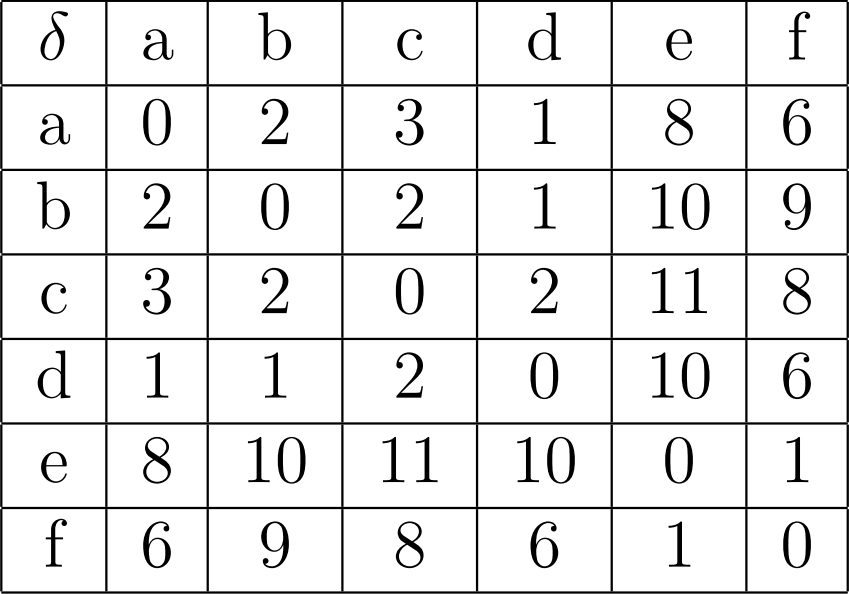
\includegraphics[scale=0.2]{macierz.png}
    \end{center}

    a) Wyznacz medoid (medoidy) dla profilu $P = \{2a, b, 3d, e, 2f\}$.
    \begin{center}
        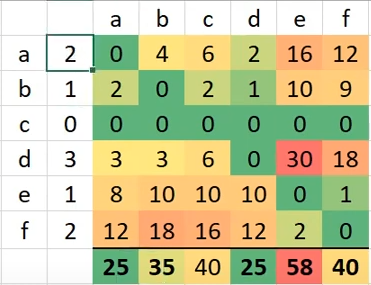
\includegraphics[scale=0.4]{medoid.png}

        Jest to $a$ lub $d$.
    \end{center}

    b) Wyznacz centroid (centroidy) dla profilu $P = \{2a, d\}$.
    \begin{center}
        \includegraphics*[scale=0.5]{centroid.png}
        
        Jest to $a$.
    \end{center}

    c) Wyznacz reprezentanta profilu $ P = \{ 2a, b, e \} $ w zbiorze $ B = \{ e,f \}$.
    \begin{center}
        \includegraphics*[scale=0.5]{reprezentant.png}

        Jest to $f$.
    \end{center}
\end{przyklad}

\begin{przyklad}
    Stosując miarę 2Dice wyznaczyć reprezentację zdefiniowanego poniżej profilu zbiorów

    Zbiór obiektów: $ U - \{ a,b,c \} $

    Zbiory profilu: $ P_1 - \{a\}, P_2 - \{b,c\}, P_3 - \{a,b\} $

    Profil: $ P = \{ 2P_1, 3P_2, P_3 \} $

    \[ P_{2Dic} = \frac{2 |X \cap Y|}{|X| + |Y|} \]

    \begin{center}
        \begin{tabular}{l|lll}
            & $P_1$ & $P_2$ & $P_3$ \\ \hline
           $P_1$ & 1 & 0 & 2/3 \\
           $P_2$ & 0 & 1 & 1/2 \\
           $P_3$ & 2/3 & 1/2 & 1
       \end{tabular}
    \end{center}

    \[ \Sigma \ \text{dla} \ P_1 = \frac{2}{2} \cdot 2 + 0 + \frac{2}{3} = 2 \frac{2}{3} \]
    \[ \Sigma \ \text{dla} \ P_2 = \frac{2 \cdot 0}{2} \cdot 2 + 3 \cdot \frac{2 \cdot 2}{2} + \frac{1}{2} = 6 \frac{1}{2} \quad \text{MAX} \]
    \[ \Sigma \ \text{dla} \ P_3 = \frac{2}{3} \cdot 2 + 3 \cdot \frac{1}{2} + 1 = \frac{4}{3} + \frac{3}{2} + 1 = \frac{23}{6} \] 

    Najlepszym reprezentantem jest $P_2$, bo dla niego uzyskano najwyższe podobieństwo dla całego profilu.
\end{przyklad}

\section{Przydatne}

Operator min - iloczyn

Operator max - suma

\begin{center}
    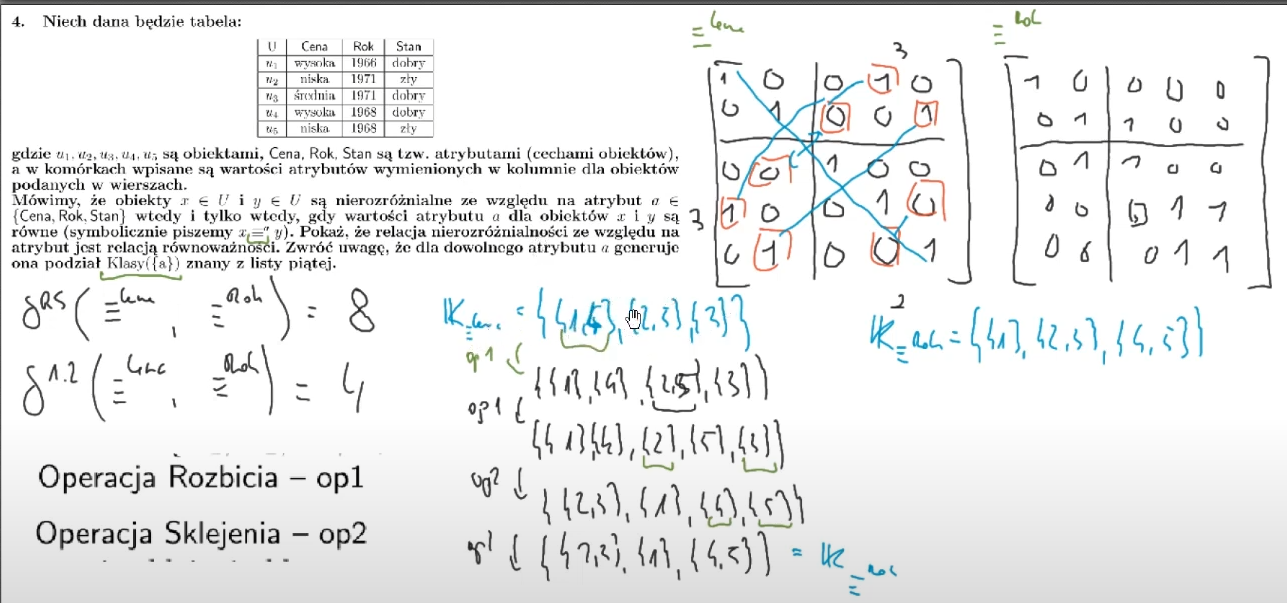
\includegraphics[scale=0.53]{atrybuty.png}
\end{center}

\end{document}